%* 
%* ------------------------------------------------------------------
%* UniversalTestReference.tex - Universal Test Program Reference Manual
%* Created by Robert Heller on Tue Aug  4 17:40:55 2009
%* ------------------------------------------------------------------
%* Modification History: $Log$
%* Modification History: Revision 1.1  2002/07/28 14:03:50  heller
%* Modification History: Add it copyright notice headers
%* Modification History:
%* ------------------------------------------------------------------
%* Contents:
%* ------------------------------------------------------------------
%*  
%*     Model RR System, Version 2
%*     Copyright (C) 1994,1995,2002-2005  Robert Heller D/B/A Deepwoods Software
%* 			51 Locke Hill Road
%* 			Wendell, MA 01379-9728
%* 
%*     This program is free software; you can redistribute it and/or modify
%*     it under the terms of the GNU General Public License as published by
%*     the Free Software Foundation; either version 2 of the License, or
%*     (at your option) any later version.
%* 
%*     This program is distributed in the hope that it will be useful,
%*     but WITHOUT ANY WARRANTY; without even the implied warranty of
%*     MERCHANTABILITY or FITNESS FOR A PARTICULAR PURPOSE.  See the
%*     GNU General Public License for more details.
%* 
%*     You should have received a copy of the GNU General Public License
%*     along with this program; if not, write to the Free Software
%*     Foundation, Inc., 675 Mass Ave, Cambridge, MA 02139, USA.
%* 
%*  
%* 
\chapter{Universal Test Program Reference}
\label{chpt:univtest:Reference}
\typeout{$Id$}

The Universal Test program is used to test the I/O ports on a USIC,
SUSIC, or SMINI node.  It is a port of the universal test program that
is shown in \cite{Chubb89} and \cite{Chubb03}.

\section{Main GUI Elements}

\subsection{Main Window}
\begin{figure}[hbpt]
\begin{centering}
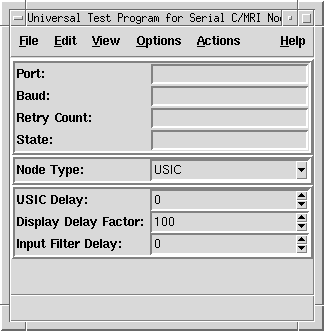
\includegraphics{UTMain.png}
\caption{The main window of the Universal Test Program}
\label{fig:ut:main}
\end{centering}
\end{figure}
The main window upon startup looks like Figure~\ref{fig:ut:main}. The
node type and initialization factors can be set.  The Display Delay
Factor is the number of hundredths of seconds between bit tests.  The
default value of 100 means a 1 second delay between output bits.  The
Input Filter Delay is the number of hundredths of seconds between bit
tests for the input port (wraparound) test.  The default value of 0
means to test as fast as possible (the program will stop if there is an
error).

\subsection{Open New Port}
\begin{figure}[hbpt]
\begin{centering}
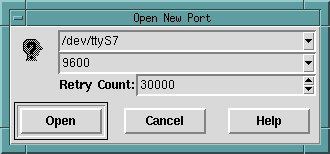
\includegraphics{UTNewCard.png}
\caption{The Open New Port dialog box of the Universal Test Program}
\label{fig:ut:new}
\end{centering}
\end{figure}
The New menu item on the File menu opens the serial port (/dev/ttySn)
the Chubb node is connected to and set the baud rate and retry count,
as shown in Figure~\ref{fig:ut:new}. The Open menu item on the File
menu opens the previously open port (if the port is currently open, it
is closed first).  The board at UA 0 is then initialized.  For USIC and
SUISC cards, it is presumed that the backplane contains just one output
card (in the first slot) for output testing, and one each output and
input card for the wraparound test (output card in the first slot and
the input card in the second slot).

\section{Tests}

There are two tests available: the output port test, which tests an output
port card and the wraparound test, which tests an input port card using
an output port card.  The output card test uses an output card LED test
plug in and lights up one LED at a time.  The wraparound uses the
wraparound cable to connect an input card to an output card and writes
bit values to the output card and reads these values on the input card
and compares what was written with what was read. These tests are
selected from the Actions menu.  

\subsection{Test Output Card}

\begin{figure}[hbpt]
\begin{centering}
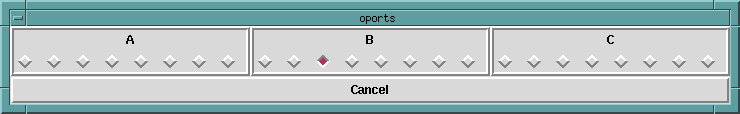
\includegraphics[width=5in]{UTOutputTest.png}
\caption{The Output Card Test Dialog Box}
\label{fig:ut:outtest}
\end{centering}
\end{figure}
The output card test displays the dialog box shown in
Figure~\ref{fig:ut:outtest}.  The lit up indicator on the dialog box
should match a corresponding LED on the output card LED test plug. The
test is repeated until canceled.

\subsection{Wraparound Test}

\begin{figure}[hbpt]
\begin{centering}
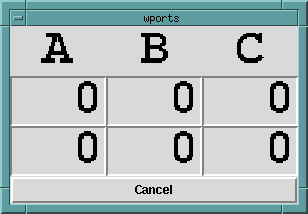
\includegraphics[width=5in]{UTWrapAround.png}
\caption{The Wraparound Test Dialog Box}
\label{fig:ut:wraptest}
\end{centering}
\end{figure}
The wraparound test displays the dialog box shown in
Figure~\ref{fig:ut:wraptest}.  The hexidecimal numbers represent the bit
pattern written to the output card.  These values are read back from the
input card and compared.  If there is a difference, the test stops and
displays the error bit pattern.

